\documentclass[a4paper, 10pt, notitlepage]{article}

\usepackage{moreverb} %para importar codigo

\usepackage[spanish,activeacute]{babel}
\usepackage{babel} %paquete de idioma

\usepackage[latin1]{inputenc}

\usepackage{pepotina} %caratula
%\usepackage{color}

%\usepackage{hyperref}
%\usepackage[all]{hypcap}

\usepackage{fancyhdr} %linea sup con comentarios

\usepackage{lscape} %para hoja apaisada

\usepackage{framed} %para crear cajas de texto

\usepackage{lastpage} %ultima pagina

\usepackage{float} %Para insertar correctamente las imagenes

%\usepackage{wrapfig} %Inclusi?n de gr?ficos al lado de texto
%\usepackage[rflt]{floatflt} %Para meter figuras flotantes entre el texto


%\usepackage{pstricks}
%\usepackage{uml} %UML

\usepackage{listings}
%\lstset{
%  breaklines=true,                                     % line wrapping on
%  language=ocl,
%  frame=ltrb,
%  framesep=5pt,
%  basicstyle=\normalsize,
%  keywordstyle=\ttfamily\color{OliveGreen},
%  identifierstyle=\ttfamily\color{CadetBlue}\bfseries,
%  commentstyle=\color{Brown},
%  stringstyle=\ttfamily,
%  showstringspaces=ture
%}

\addtolength{\topmargin}{-50pt} 
\addtolength{\textwidth}{105pt}
\addtolength{\textheight}{120pt}
\addtolength{\oddsidemargin}{-50pt}

%\newcommand{\minix}{\textsl{minix }}

%%% Encabezado y pie de p'agina
\pagestyle{fancy}
\fancyhead[LO]{Sistemas Operativos}
\fancyhead[C]{}
\fancyhead[RO]{P\'agina \thepage\ de \pageref{LastPage}}
\renewcommand{\headrulewidth}{0.4pt}
\fancyfoot{}

\newcommand{\quota}{\textit{quota }}
\newcommand{\quantum}{\textit{quantum }}
\newcommand{\quantums}{\textit{quantums }}
\newcommand{\rr}{\textit{Round-Robin }}
\newcommand{\mfq}{\textit{Multilevel Feedback Queue }}
\newcommand{\cs}{\textit{context switch }}
\newcommand{\wt}{\textit{waiting time }}
\newcommand{\ta}{\textit{turnaround }}
\newcommand{\latencia}{\textit{latencia }}


\def\falta#1{ \begin{framed}	\begin{center} \hspace{1cm} \Large FALTA \normalsize #1 \hspace{1cm} \end{center} \end{framed}}


\def\imagen#1#2{\vskip0.5cm
\begin{center}
\includegraphics[scale=#1]{#2}
\end{center}}

\newenvironment{mydescription}[1]
  {\begin{list}{}%
   {\renewcommand\makelabel[1]{##1\hfill}%
   \settowidth\labelwidth{\makelabel{#1}}%
   \setlength\leftmargin{\labelwidth}
   \addtolength\leftmargin{\labelsep}}}
  {\end{list}}

\begin{document}

\universidad{Universidad de Buenos Aires}
\facultad{Facultad de Ciencias Exactas y Naturales}
\departamento{Departamento de Computaci\'on}
\materia{Sistemas Operativos}
\resumen{SOScrabel versi\'on web-social-online-multijugador-twitter-facebook de su cl\'asico juego de mesa Scrable.}
\keys{pthreads, sockets, mutex, server, client, http, tcp, scrabel}
\titulo{Tp2: Pthreads}
\subtitulo{SOScrabel ueb tu point ou}
\grupo{N\'umero de grupo: 12}
\fecha{1er Cuatrimeste 2011}
\footspace{1cm}
\integrante{Dominguez, Pablo Sebastian}{108/05}{pablo.sebastian.dominguez@gmail.com}
\integrante{Engler, Christian Alejandro}{314/05}{caeycae@gmail.com}

%caratula	
\maketitle{}

\tableofcontents

\newpage



\part{Entendiendo el Simulador simusched}

\section{Ejercicio 1}

Implementamos el m\'etodo TaskCon que simula ser una tarea interactiva, que recibe los par\'ametros \verb|n|, \verb|bmin| y \verb|bmax|.

Realiza \verb|n| llamadas bloqueantes de duraci\'on entre \verb|bmin| y \verb|bmax|.

\begin{framed}
\begin{verbatimtab}
void TaskCon(vector<int> params) { // params: 3
	int n = params[0];
	int bmin = params[1];
	int bmax = params[2];
	
	for( int i = 0; i < n ; i++ ) {
		int time = bmin;
		if(bmin != bmax)
			time = (rand()%(bmax-bmin+1))+bmin;
		uso_IO(time);
	}
}
\end{verbatimtab}
\end{framed}

\section{Ejercicio 2}

Escribimos un lote de 3 tareas distintas: una intensiva en CPU y las otras dos de tipo interactivo. 
El lote lo escribimos en \verb|ejercicio2.tsk|.

\begin{framed}
\begin{verbatim}
# FILE ejercicio2.tsk
TaskCPU 10
@1
TaskCon 10 1 4
@3
TaskCon 7 1 3
\end{verbatim}
\end{framed}

Luego ejecutamos Simusched con Scheduler FCFS con los siguientes parametros:

\begin{verbatim}
./simusched ejercicio2.tsk 1 SchedFCFS | python graphsched.py > ejercicio2.png
\end{verbatim}

Y obtuvimos el siguiente diagrama de Gantt.

\begin{figure}[H]
  \centering
    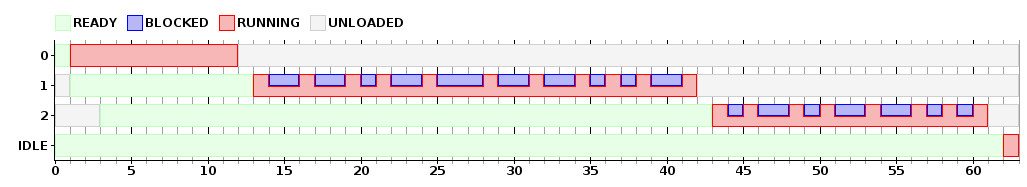
\includegraphics[width=1\textwidth]{img/ejercicio2.png}
    \caption{Una tarea de uso intensivo del procesador y dos interactivas con Scheduling FCFS.}
\end{figure}

Se ve en el diagrama que las tareas se ejecutan en el orden de llegada y que al no existir desalojo en FCFS las tareas mantienen el procesador incluso al estar bloqueadas.


\newpage
\section{Otras modificaciones}

Ahora como el server es multithread cuando el cliente finaliza su conexi\'on con el servidor, tanto por una falla como por decisi\'on propia, no debe finalizar el juego. Para lo cual modificamos el ciclo de cada thread que ante la finalizaci\'on solamente corta el thread de ese jugador.

Dado el comportamiento que le estamos dando al juego con esta modificaci\'on, el backend ahora no finaliza, este se queda escuchando constantemente el ingreso o egreso de clientes.

-//TODO Ver cuando liberar los mutex.

\end{document}
